\chapter{BIODATA PENULIS}
\begin{wrapfigure}{l}{0.4\textwidth}
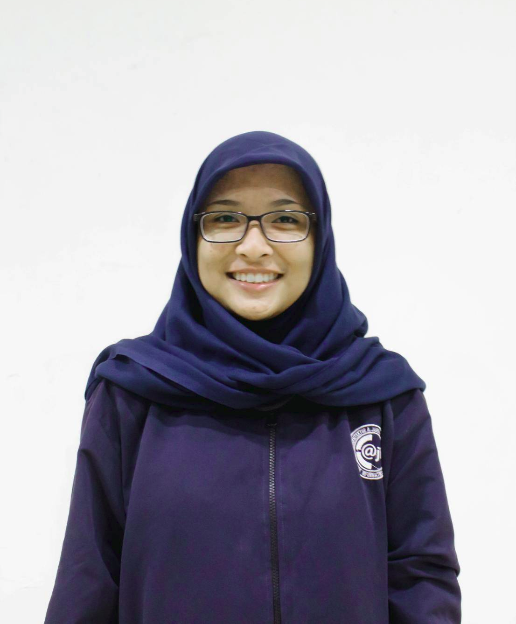
\includegraphics[height=0.3\textheight]{biodata/foto1.png}
\end{wrapfigure}

\textbf{Rohana Qudus}, lahir di Gresik tanggal 7 Februari 1998. Penulis merupakan anak kedua dari 2 bersaudara. Penulis telah menempuh pendidikan formal TK Dharmawanita Gresik, SD Muhammadiyah 2 Gresik (2004-2010), SMP Negeri 1 Gresik (2010-2013) dan SMA Negeri 1 Gresik (2013-2015). Penulis melanjutkan studi kuliah program sarjana di Departemen Informatika ITS. 

Selama berkuliah di Departemen Informatika ITS, penulis  pernah menjadi asisten dosen dan praktikum untuk mata kuliah Sistem Operasi (2017) dan Jaringan Komputer(2018). Selama menempuh perkuliahan penulis juga aktif di kegiatan organisasi dan kepanitiaan diantaranya menjadi Staf Departemen Media Informasi HMTC ITS, Staf Departemen Informasi Informasi Media BEM FTIF ITS, Staf Ahli Departemen Media Informasi HMTC ITS, Staf Website dan Kesekretariatan Schematics 2016, dan Staf Ahli 3D Schematics 2017. Penulis dapat dihubungi melalui surel di \\ \texttt{rohanaq27@gmail.com}.

\chapter{BIODATA PENULIS}
\begin{wrapfigure}{l}{0.4\textwidth}
	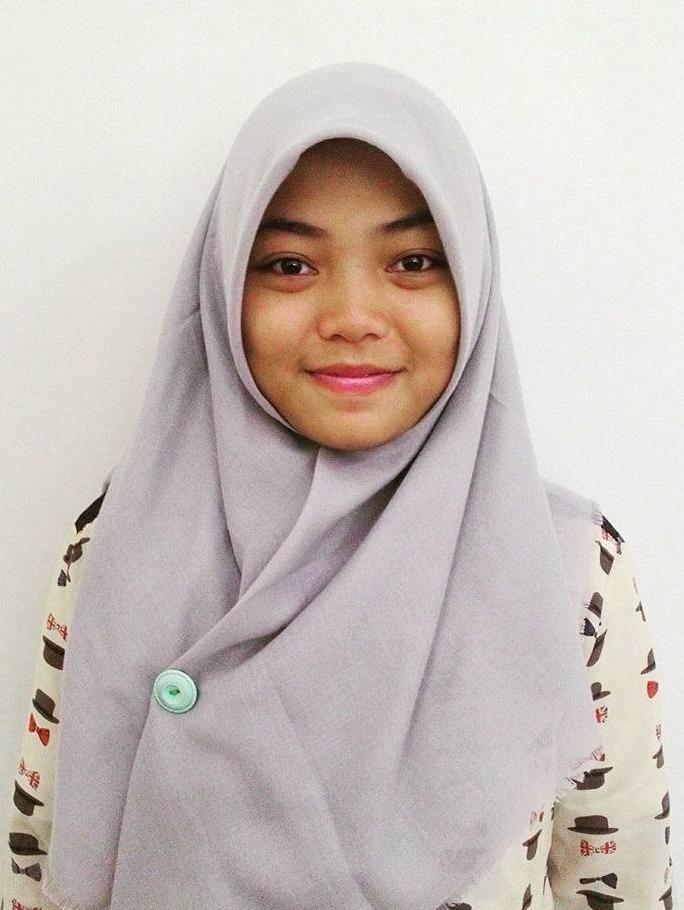
\includegraphics[height=0.3\textheight]{biodata/foto.jpg}
\end{wrapfigure}
\textbf{Rafi R. Ramadhan}, lahir di Gresik tanggal 7 Februari 1998. Penulis merupakan anak kedua dari 2 bersaudara. Penulis telah menempuh pendidikan formal TK Dharmawanita Gresik, SD Muhammadiyah 2 Gresik (2004-2010), SMP Negeri 1 Gresik (2010-2013) dan SMA Negeri 1 Gresik (2013-2015). Penulis melanjutkan studi kuliah program sarjana di Departemen Informatika ITS. 

Selama berkuliah di Departemen Informatika ITS, penulis  pernah menjadi asisten dosen dan praktikum untuk mata kuliah Sistem Operasi (2017) dan Jaringan Komputer(2018). Selama menempuh perkuliahan penulis juga aktif di kegiatan organisasi dan kepanitiaan diantaranya menjadi Staf Departemen Media Informasi HMTC ITS, Staf Departemen Informasi Informasi Media BEM FTIF ITS, Staf Ahli Departemen Media Informasi HMTC ITS, Staf Website dan Kesekretariatan Schematics 2016, dan Staf Ahli 3D Schematics 2017. Penulis dapat dihubungi melalui surel di \\ \texttt{rohanaq27@gmail.com}.
